\chapter{Geometric Groups}\label{c9}

Connell\pageoriginale and Hollingsworth \cite{20} introduced the
notion of geometric\break group in the hope of proving the topological
invariance of Whitehead torsion. Although they did not succeed at that
time, their concept was revived by F. Quinn \cite{84} who showed that
it is a useful framework in which to prove ``control theorems'' in
topology. 

A \textit{Geometric} group $G$ on a metric space $X$ is a finite
sequence 
$$
x_1, \ldots , x_n
$$ 
of points in $X$; $G$ also dentoes the
free abelian group equipped with the ordered basis $x_1, \ldots ,
x_n$. (More precisely, the basis is $(1, x_1), (2, x_2), \ldots ,\break (n,
x_n)$; if $i \neq j$ but $x_i = x_j$, we will consider $x_i$ and $x_j$
to be distinct elements in $G$.)

\begin{remark*}
  One can similarly define the concept of geometric $R$-module over
  $X$ where $R$ is a fixed ring. This notion is particularly useful
  whrn $R= \mathbb{Z} \Pi$ where $\Pi$ is a discrete group. But, for
  the present, we will stick to the case $\Pi = 1$; i.e., $R= \mathbb{Z}$.
\end{remark*}

Let $G_1$ and $G_2$ be two geometric groups with bases $\{ x_i\}$ and
$\{y_j\}$, respectively, and $f: G_1 \to G_2$ be a homomorphism. It
determines a set valued function $C(f)$ defined by 
$$
  C(f) (x_i)= \{ y_i \mid y_i ~\text{has nonzero coefficient in}~ f(x_i)\}.
$$

The \textit{diameter} of $f$, denoted diam $f$, is defined to be
$$
\sup\limits_{i} ~diameter~ (\{ x_i \} \cup C(f)(x_i)).
$$

\begin{defi}\label{c9:defi9.1}
  A homomorphism $f: G \to G$ is a $\delta$-endomorphism if diam $f
  \leq \delta$. And $f$ is a $\delta$-automorphism if $f$ is
  invertible and both $f$ and $f^{-1}$ are $\delta$-endomorphisms.
\end{defi}

Assume from now on that $X$ is compact, locally contractible and
arc-connected; e.g., $X$ could be either a finite (connected)
simplicial complex or a compact (connected) manifold. Fix a pair of
positive real numbers $\delta_1 > \delta_0 > 0$ such that the
following metric connectedness conditions are satisfied.

\begin{enumerate}
\item Any two points $x, y \in X$ with $d(x, y) \leq \delta_0$ are
  connected by an arc of diameter $\leq \delta_1$.
  \item Any\pageoriginale closed curve of diameter $\leq 2 \delta_1$ is null homotopic.
\end{enumerate}

Let $\Gamma = \pi_1 (X, *)$ and $M_n (\mathbb{Z} \Gamma)$ be the ring
of all $n \times n$ matrices with entries in $\mathbb{Z}\Gamma$. Given
any $\delta_0$-endomorphism $f: G \to G$ of a geometric group on $X$,
there is associated an element $\hat{f} \in M_n (\mathbb{Z}\Gamma)$
defined as follows. Let $x_1, x_2, \ldots , x_n \in X$ be the basis of
$G$. The construction of $\hat{f}$ depends on a choice of paths
$\alpha_1, \ldots , \alpha_n$ in $X$ such that $\alpha_i$ connects $*$
to $x_i$. Let $f_{ij} \in \mathbb{Z}$ denote the coefficient of $x_i$
in the expression of $f(x_j)$; i.e.,
$$
f(x_j) = \sum_i f_{ij} x_i.
$$

For each pair of indices $i$, $j$ such that $d(x_i, x_j) \leq
\delta_0$, pick a path $\gamma_{ij}$ connecting $x_j$ to $x_i$ and
such that diameter $\gamma_{ij} \leq \delta_1$. This is possible
because of condition 1. (The construction of $\hat{f}$ will be
independent of this choice.) We now define the $i$, $j$ entry of
$\hat{f}$ by the formula
$$
\hat{f}_{ij}=
\begin{cases}
  f_{ij} \alpha_i^{-1} * \gamma_{ij} * \alpha_j & \text{where}~ f_{ij}
  \neq 0\\
  0 & \text{otherwise}
\end{cases}
$$
where $\alpha_i^{-1} * \gamma_{ij} * \alpha_j$ is the homotopy class
of the closed loop gotten by concatenating the paths $\alpha_j$,
$\alpha_{ij}$, $\alpha_i^{-1}$. Condition 2 shows that $\hat{f}$ is
independent of the choice $\gamma_{ij}$. We now examine its dependence
on $\{ \alpha_i\}$. Suppose new paths $\{\beta_i \}$ are chosen and
let $\gamma_i \in \pi_1 (X, *)$ be the homotopy class represented by
the closed loop $\beta_i^{-1}* \alpha_i$. Let $D$ denote the diagonal
$n \times n$ matrix defined by $D_{ij}= \gamma_i$. A consideration of
Figure 7 yields the first result below.

\begin{figure}[H]
  \centering{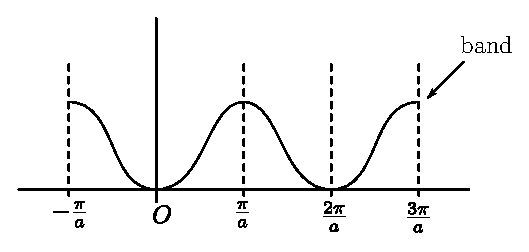
\includegraphics{vol86-figures/fig7.eps}\\
  Figure 7}
\end{figure}
 
\begin{lemma}\label{c9:lem9.2}
  If\pageoriginale we choose new paths $\beta_i$ as above, then the matrix
  associated to $f$ changes from $\hat{f}$ to $D\hat{f} D^{-1}$.
\end{lemma}

\begin{lemma}\label{c9:lem9.3}
  Suppose $f, g: G \to G$ are two $\delta_0/3$-endomorphisms of the
  geometric group $G$. Then their composition $f \circ g$ is a
  $\delta_0$-endomorphisms of the geometric group $G$. Then their
  composition $f \circ g$ is a $\delta_0$-endomor\-phism of $G$ and
  $\widehat{f \circ g}= \hat{f} \hat{g}$. 
\end{lemma}

\begin{proof}
  It is clear that $f \circ g$ is a $\delta_0$-endomorphism. Fix a
  choice of paths $\alpha_i$ and $\gamma_{ij}$ as before. Because of
  conditions 1 and 2, the concatenation $\gamma_{ik}* \gamma_{kj}$ is
  homotopic to $\gamma_{ij}$. Consider the following calculation
  \begin{align*}
    (\hat{f} \hat{g})_{ij} & = \sum_k \hat{f}_{ik} \hat{g}_{kj}\\
    & = \sum_k f_{ik} (\alpha_i^{-1} * \gamma_{ik} * \alpha_k) g_{kj}
    (\alpha_k ^{-1} * \gamma_{kj} * \alpha_j)\\
    & = \sum_k f_{ik} g_{kj} (\alpha_i^{-1} * \gamma_{ik} * \gamma_{kj}
      * \alpha_j)\\
      & = \left(\sum_k f_{ik} g_{kj} \right) \alpha_i^{-1} *
      \gamma_{ij} * \alpha_j\\
      & = (fg)_{ij} \alpha_i^{-1} * \gamma_{ij} * \alpha_j\\
      & = (\widehat{f \circ g})_{ij}. \qquad \text{Q.E.D.}
  \end{align*}
\end{proof}

\begin{remark*}
  If $f_1, f_2, \ldots , f_n$ are endomorphisms of $G$ such that diam
  $f_i \leq a$ for each $i$, then diam $f_n \circ \ldots \circ f_1\leq
  2 na$.
\end{remark*}

\begin{coro}\label{c9:coro9.4}
  If $f: G \to G$ is a $\delta_0/3$-automorphism, then $\hat{f} \in
  GL_n (\mathbb{Z}\Gamma)$ and determines a well defined element
  in $Wh (\Gamma)$, which we also denote by $\hat{f}$.
\end{coro}

\begin{proof}
  Apply Lemma \ref{c9:lem9.3} with $g = f^{-1}$. Then
  \begin{align*}
    \widehat{id} & = \widehat{f \circ g} = \hat{f} \circ
    \hat{g} ~\text{and}\\
    \widehat{id} & = \widehat{g \circ f} = \hat{g} \circ \hat{f}.
  \end{align*}
  But clearly $\widehat{id} = id$. Therefore, $\hat{f}$ is
  invertible. And its value in $Wh(\Gamma)$ is independent of the
  choice of the paths $\alpha_i$, because of Lemma \ref{c9:lem9.2}.
\end{proof}
